\documentclass[main]{subfiles}
\begin{document}

%@@@@@@@@@@@@@@@@@@@@@@@@@@@@@@
% summarizes lecture 
% author:

\section{Parametric Models} 
Unfortunately, in pattern recognition applications we rarely if ever have this kind of complete knowledge about the probabilistic structure of the problem. In a typical case we merely have some vague, general knowledge about the situation, together with a number of design samples or training data - particular representatives of the patterns we want to classify. The problem, then, is to find some way to use this information to design or train the classifier.\\
In statistics, a parametric model or parametric family or finite-dimensional model is a family of distributions that can be described using a finite number of parameters. These parameters are usually collected together to form a single k-dimensional parameter vector \(\pl{\theta = (\theta_1, \theta_2, \ldots, \theta_k).}\)\\\\
If we know the number of parameters in advance and our general knowledge about the problem permits us to parameterize the conditional densities, then the severity of these problems can be reduced significantly.
The problem of parameter estimation is a classical one in statistics, and it can be
approached in several ways. We shall consider two common and reasonable procedures, maximum likelihood estimation and Bayesian estimation.
\subsection{Maximum Likelihood Estimation}
Likelihood of the data set: \(\printlatex{P(\mathcal{X}|\theta_y) = \prod\limits_{i\leq n_y}p(x_i|\theta_y)}\)\\
\textbf{Estimation principle:} Select the parameter \(\pl{\hat\theta_y}\) which maximizes
the likelihood, i.e., the probability of the data given the parameter:
\[\pl{\hat\theta_y = \argmax\limits_{\theta_y} P\{X_y |\theta_y \}}\]
The random variable \(\pl{\hat\theta_y (\mathcal{X}_y )}\) is called an estimator for the parameter \(\pl{\theta}\).\\
\textbf{Procedure:} Find the extremum of the log-likelihood function:
\[\pl{\Lambda(\theta) \triangleq \nabla_{\theta_y} \log P\{\mathcal{X}|\theta_y\}  = \frac{\partial}{\partial \theta_y} \sum\limits_{i\leq n} \log p(x_i|\theta_y) = 0}\]
\subsubsection{Remarks on Maximum Likelihood estimators}
\paragraph{Bias of an estimator} \(\pl{bias(\hat\theta_n) = \E[\hat\theta_n] - \theta}\)
The bias measures how much the expected value of the estimator deviates from the true parameter value. The design of unbiased estimators (\(\pl{\E[ \hat\theta_n ] = \theta)}\) and bias reduction has been considered as a goal of statistics, although the work of Stein has shown that there exists biased estimators which are better in the least squares sense than any unbiased estimator.
\paragraph{Consistent estimator}
A point estimator \(\pl{\hat\theta_n}\) of a parameter \(\pl{\theta}\) is consistent if \(\pl{\hat\theta_n \overset{P}{\rightarrow} \theta}\), i.e.,
\[\pl{\forall \epsilon P\{|\hat\theta_n - \theta| > \epsilon\} \overset{n\rightarrow\infty}{\rightarrow} 0}\]
\paragraph{Efficiency} ML estimators are asymptotically efficient estimators, i.e.,
\[\pl{\lim\limits_{n\rightarrow\infty}\left(\V[\hat\theta^{ML} (x_1,\ldots,x_n)] I(\theta)\right)^{-1} = 1,~~I = \V\left[\frac{\partial\log P(x|\theta)}{\partial \theta}\right]}\]
\subsubsection{Rao-Cramer Inequality}
The Rao-Cramer inequality states that the variance of an estimator is bounded from below by the inverse Fisher information. The fisher information is denoted by:
\[\pl{I(\theta) 
=
\overbrace{\V\left[\frac{\partial \log P(x;\theta)}{\partial \theta}\right]}^{\hidewidth\text{Variance of the score function}\hidewidth}
= \underbrace{\E\left[\left(\frac{\partial \log P(x;\theta)}{\partial\theta}
  \right)^2\right]}_{\hidewidth\text{Expected value of the observed information}\hidewidth}
= -\E\left[ \frac{\partial^2 \log P(x;\theta)}{\partial\theta^2} \right]}\]
Let \(\hat\theta(X_1 , \ldots , X_n )\) be an unbiased estimator of \(\theta\).
then the Rao Cramer inequality holds for the class of unbiased estimators:
\[\pl{\int (\theta-\hat\theta)^2 P(x_1,\ldots,x_n;\theta)dx_1\ldots dx_n \leq \frac{1}{I(\theta)}}\]
\subsubsection{Convergence of Maximum Likelihood Estimators}
The Maximum Likelihood estimator converges (in distribution; Central Limit Theorem) to the best model \(\theta_0\) as \(n\rightarrow \infty\) (Asymptotic normality).
\begin{align}
\pl{\sqrt{n} (\hat\theta^{ML}_n - \theta_0) &\overset{n\rightarrow \infty}{\rightarrow} \mathcal{N}(0,J^{-1}(\theta_0)I(\theta_0)J^{-1}(\theta_0))}\\
J(\theta) &= - \E\left[\frac{\partial^2 \log P(x|\theta)}{\partial \theta^2}\right]\\
I(\theta) &= - \V\left[\frac{\partial \log P(x|\theta)}{\partial \theta}\right]\\
\end{align}
\todo[inline]{Do we need the proof for that?}
\subsection{Bayesian Learning (batch/online)}
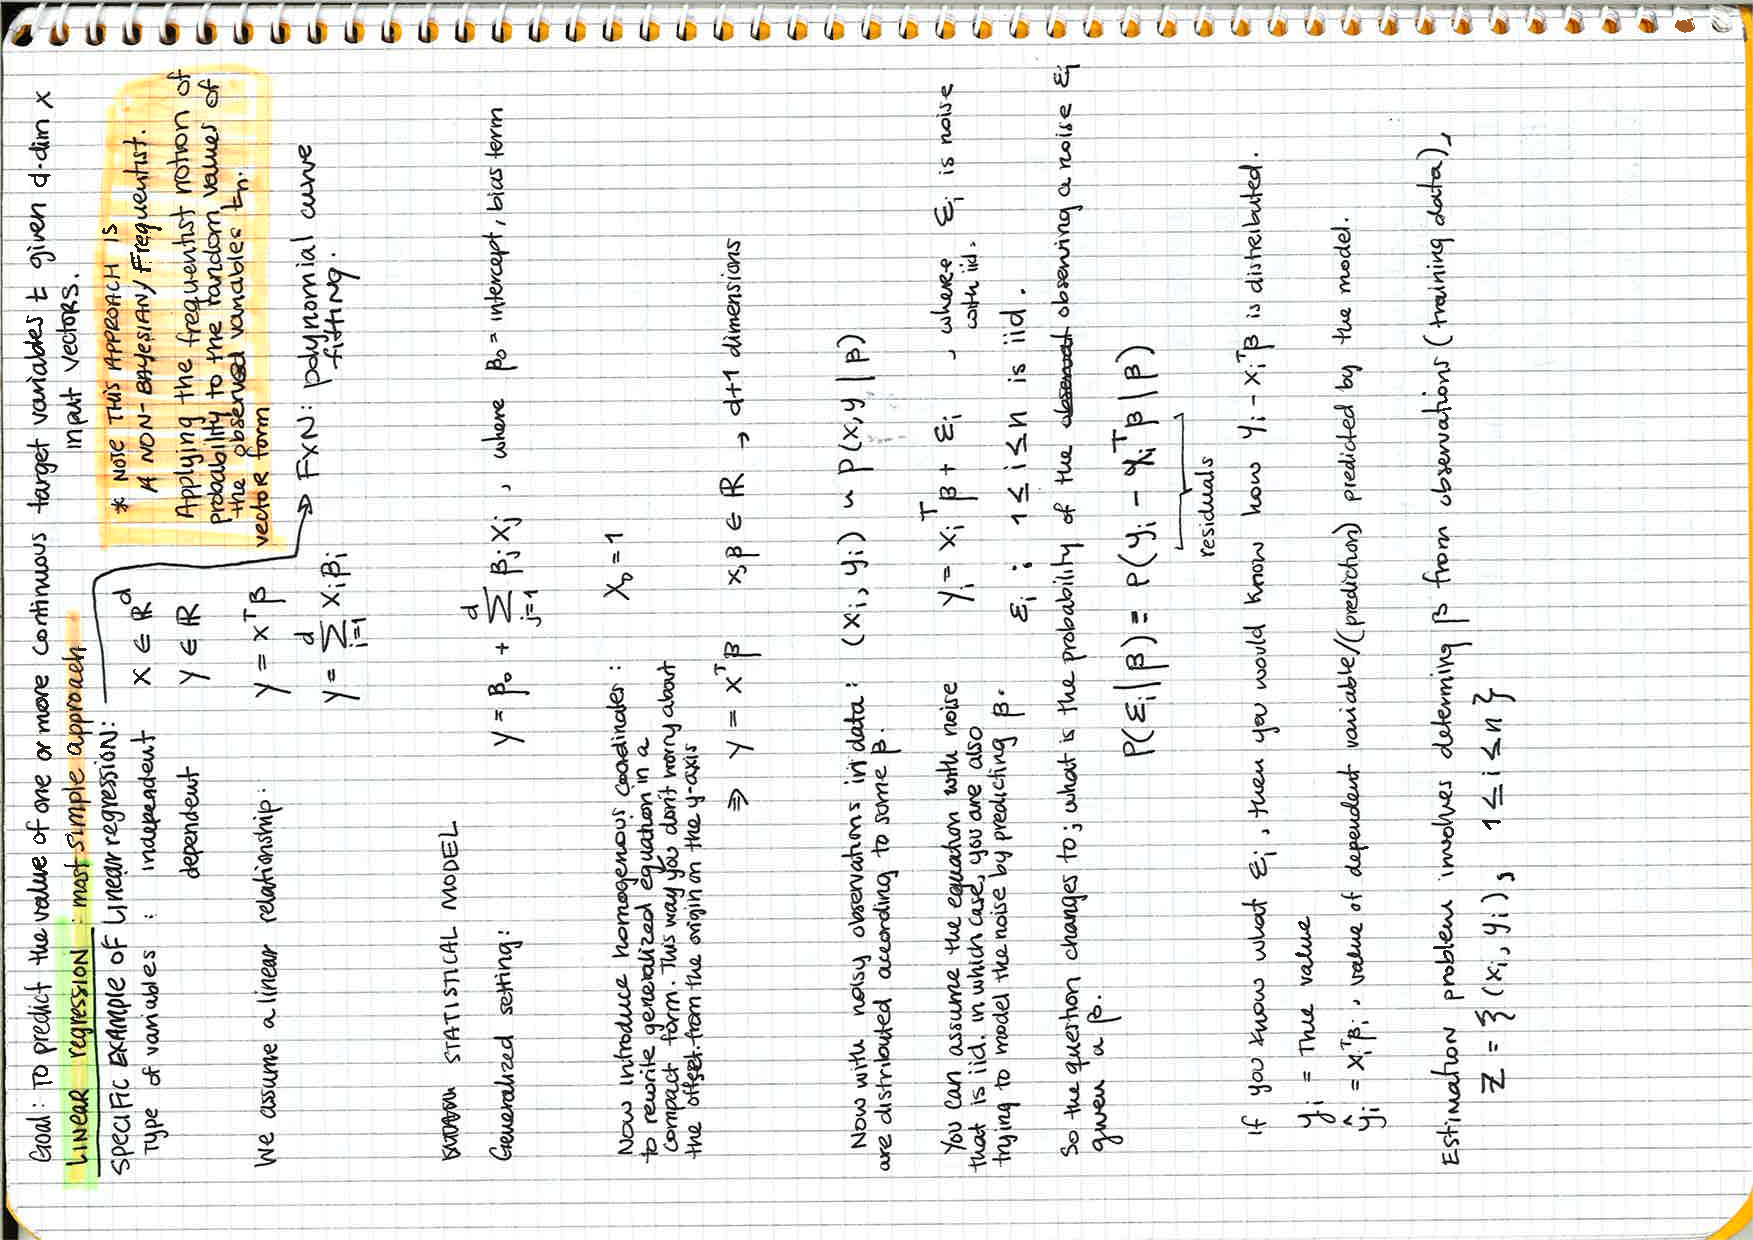
\includepdf[pages=1,angle=-90]{figs/bayesian/1543_001.pdf}
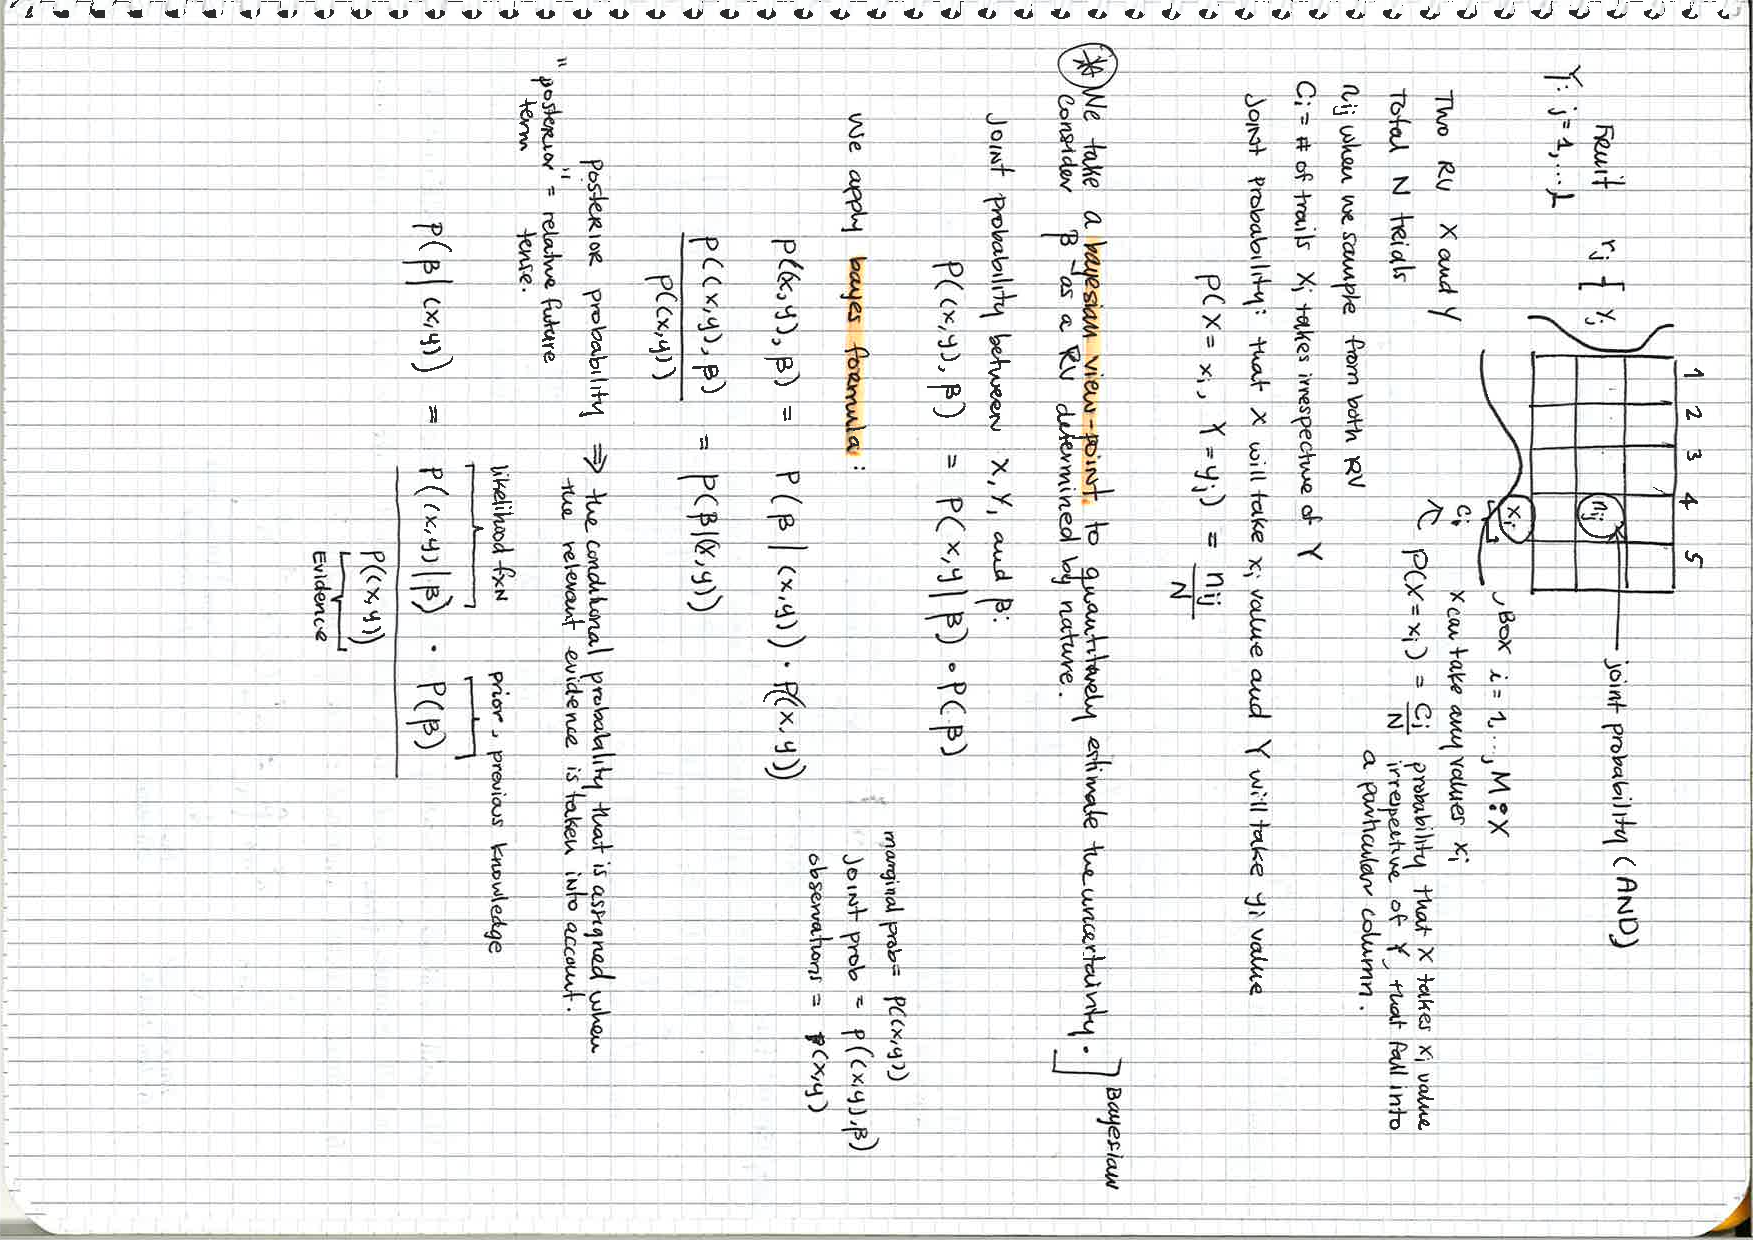
\includepdf[pages=1,angle=90]{figs/bayesian/1544_001.pdf}
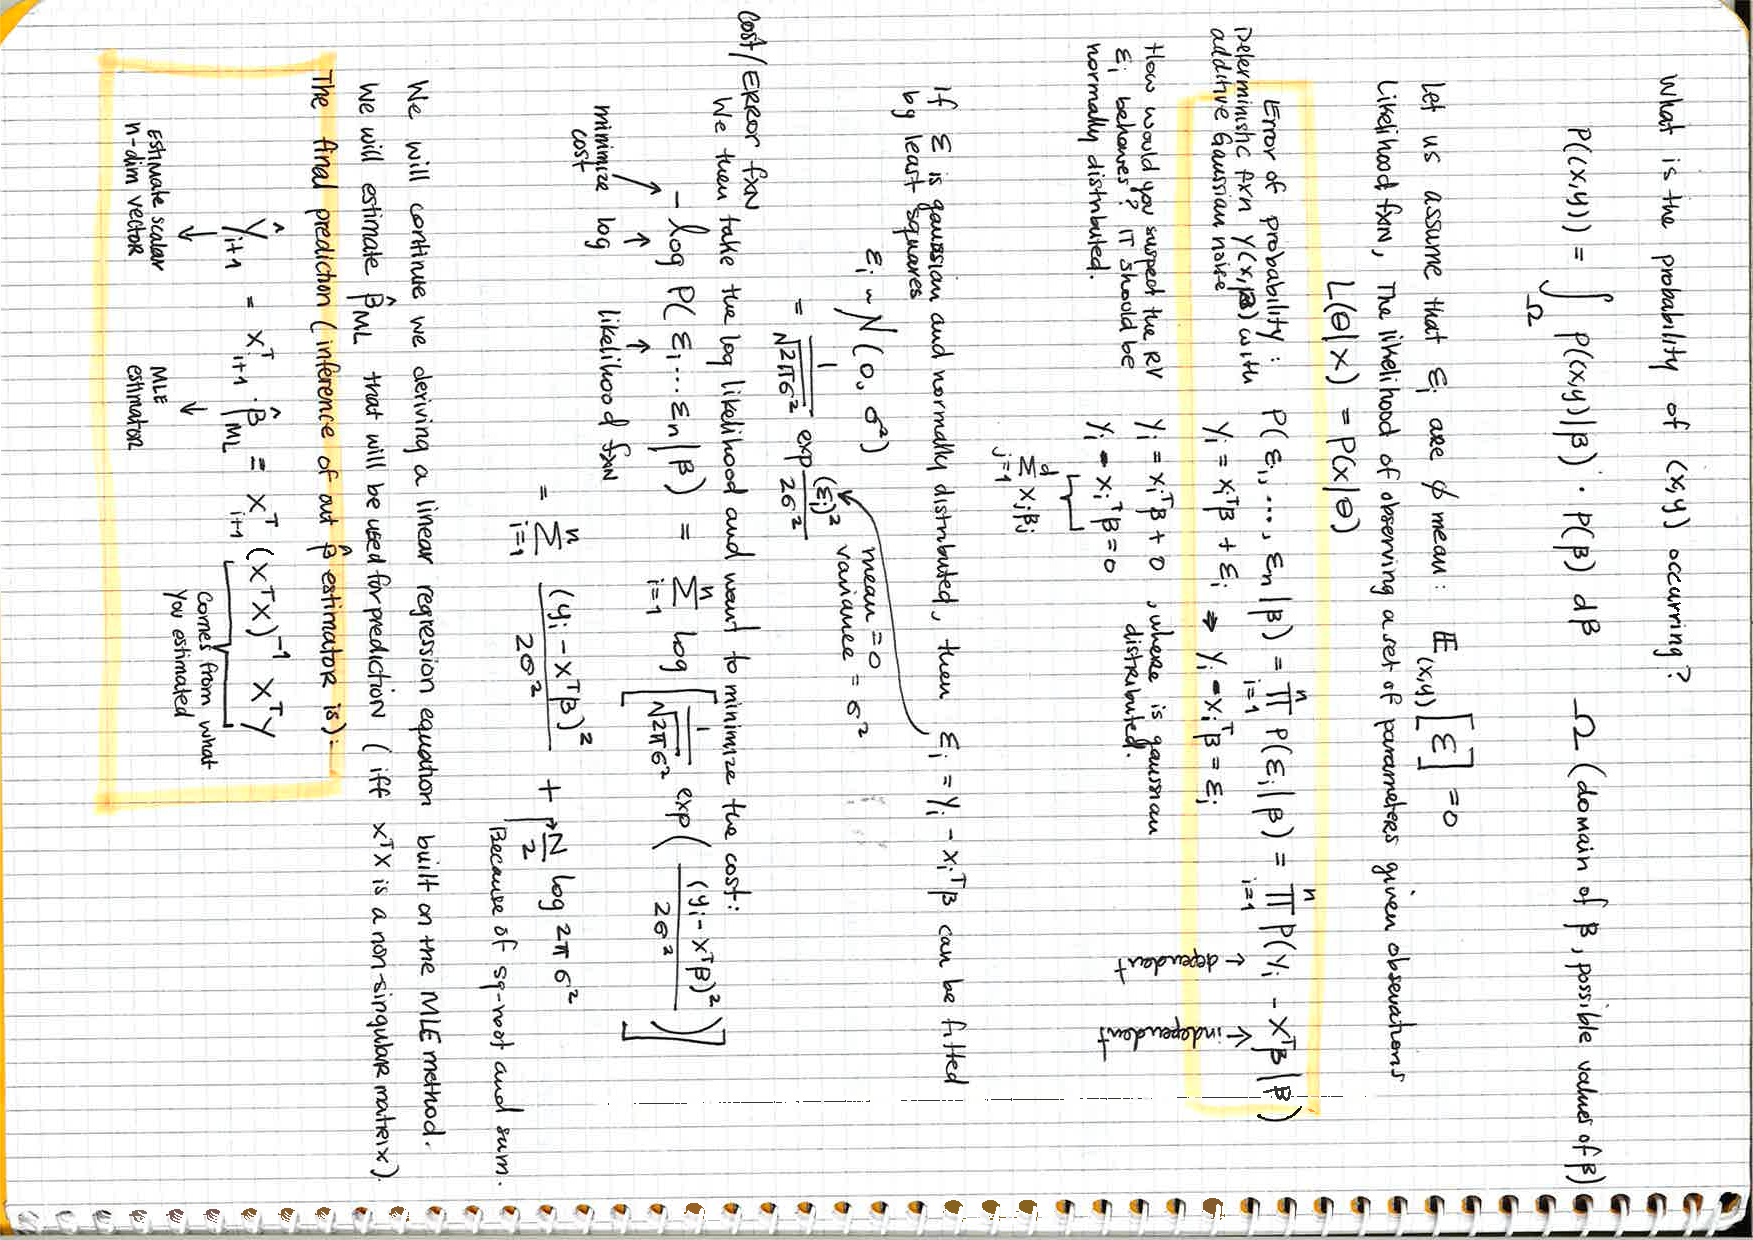
\includepdf[pages=1,angle=90]{figs/bayesian/1545_001.pdf}
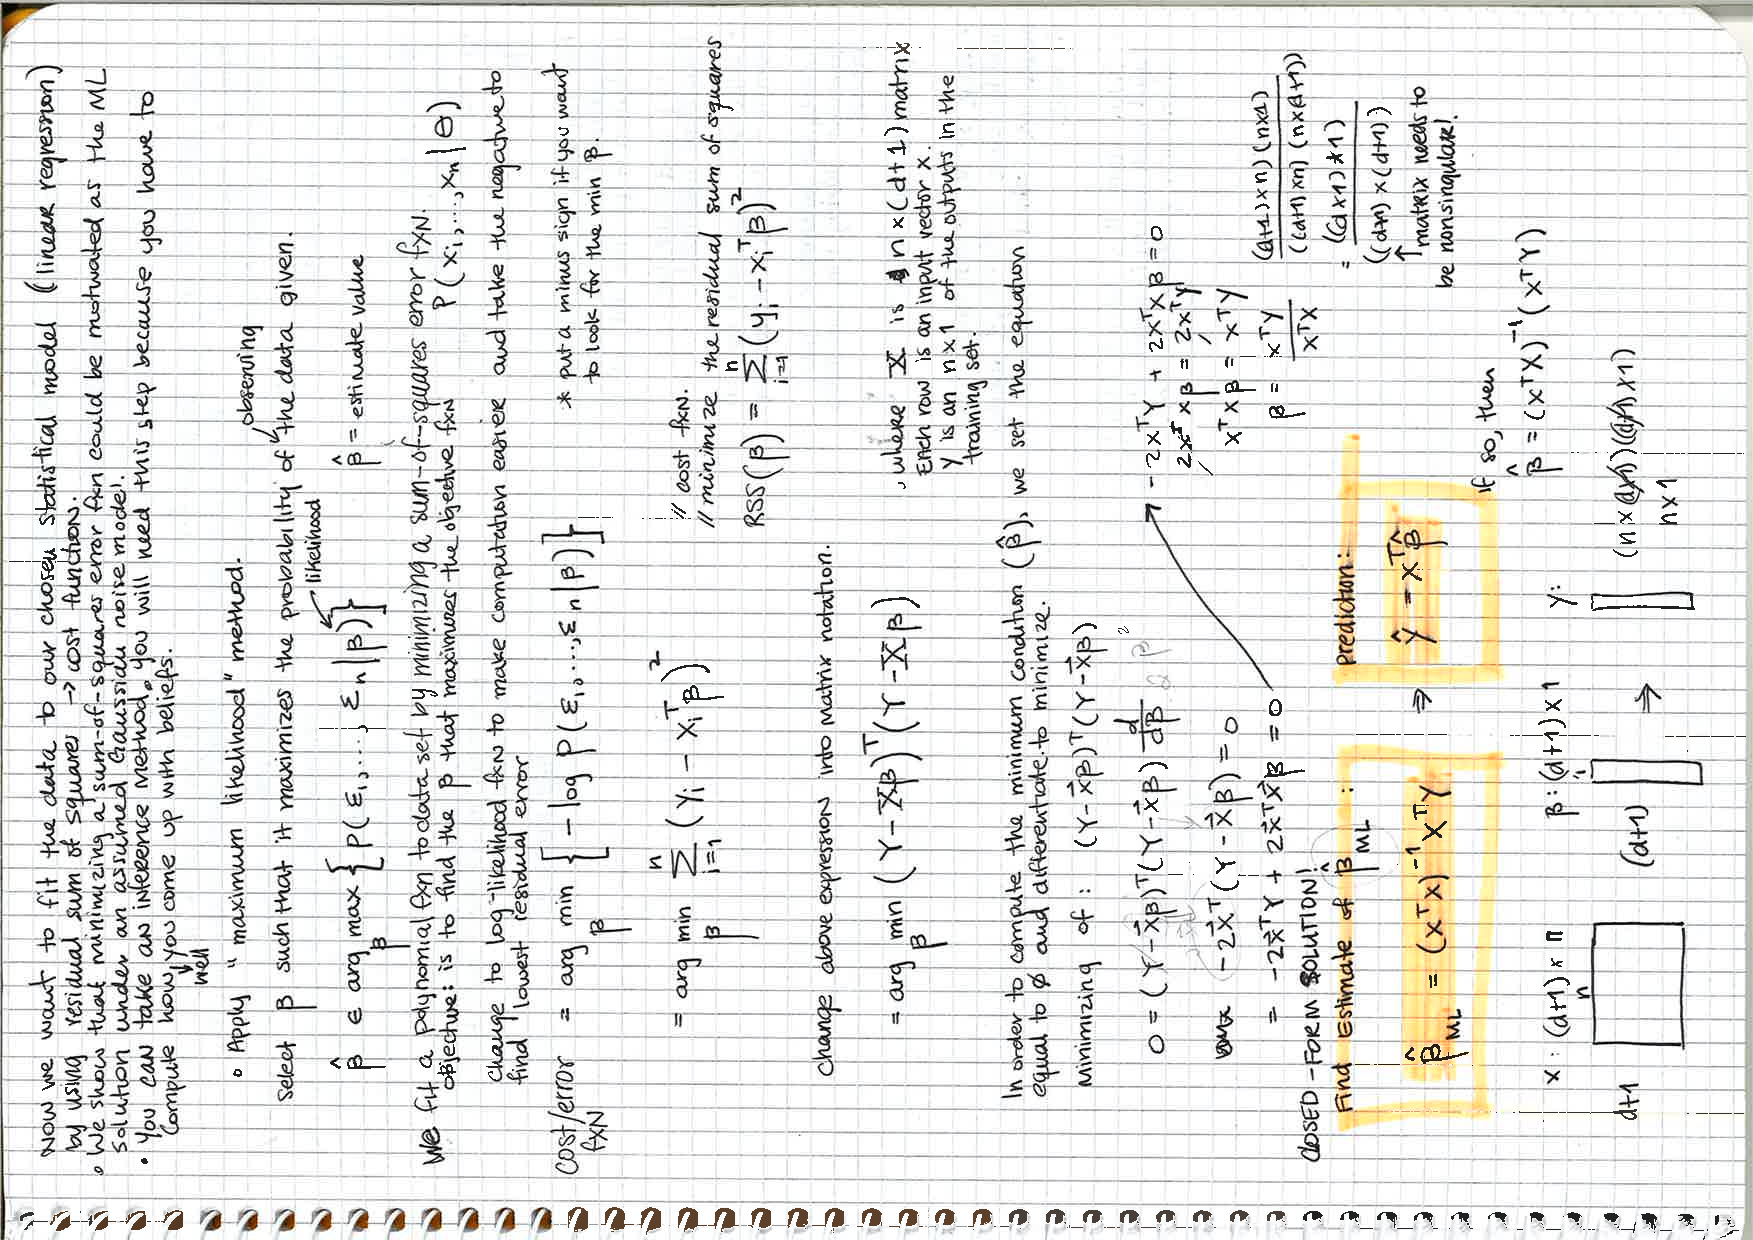
\includepdf[pages=1,angle=-90]{figs/bayesian/1546_001.pdf}
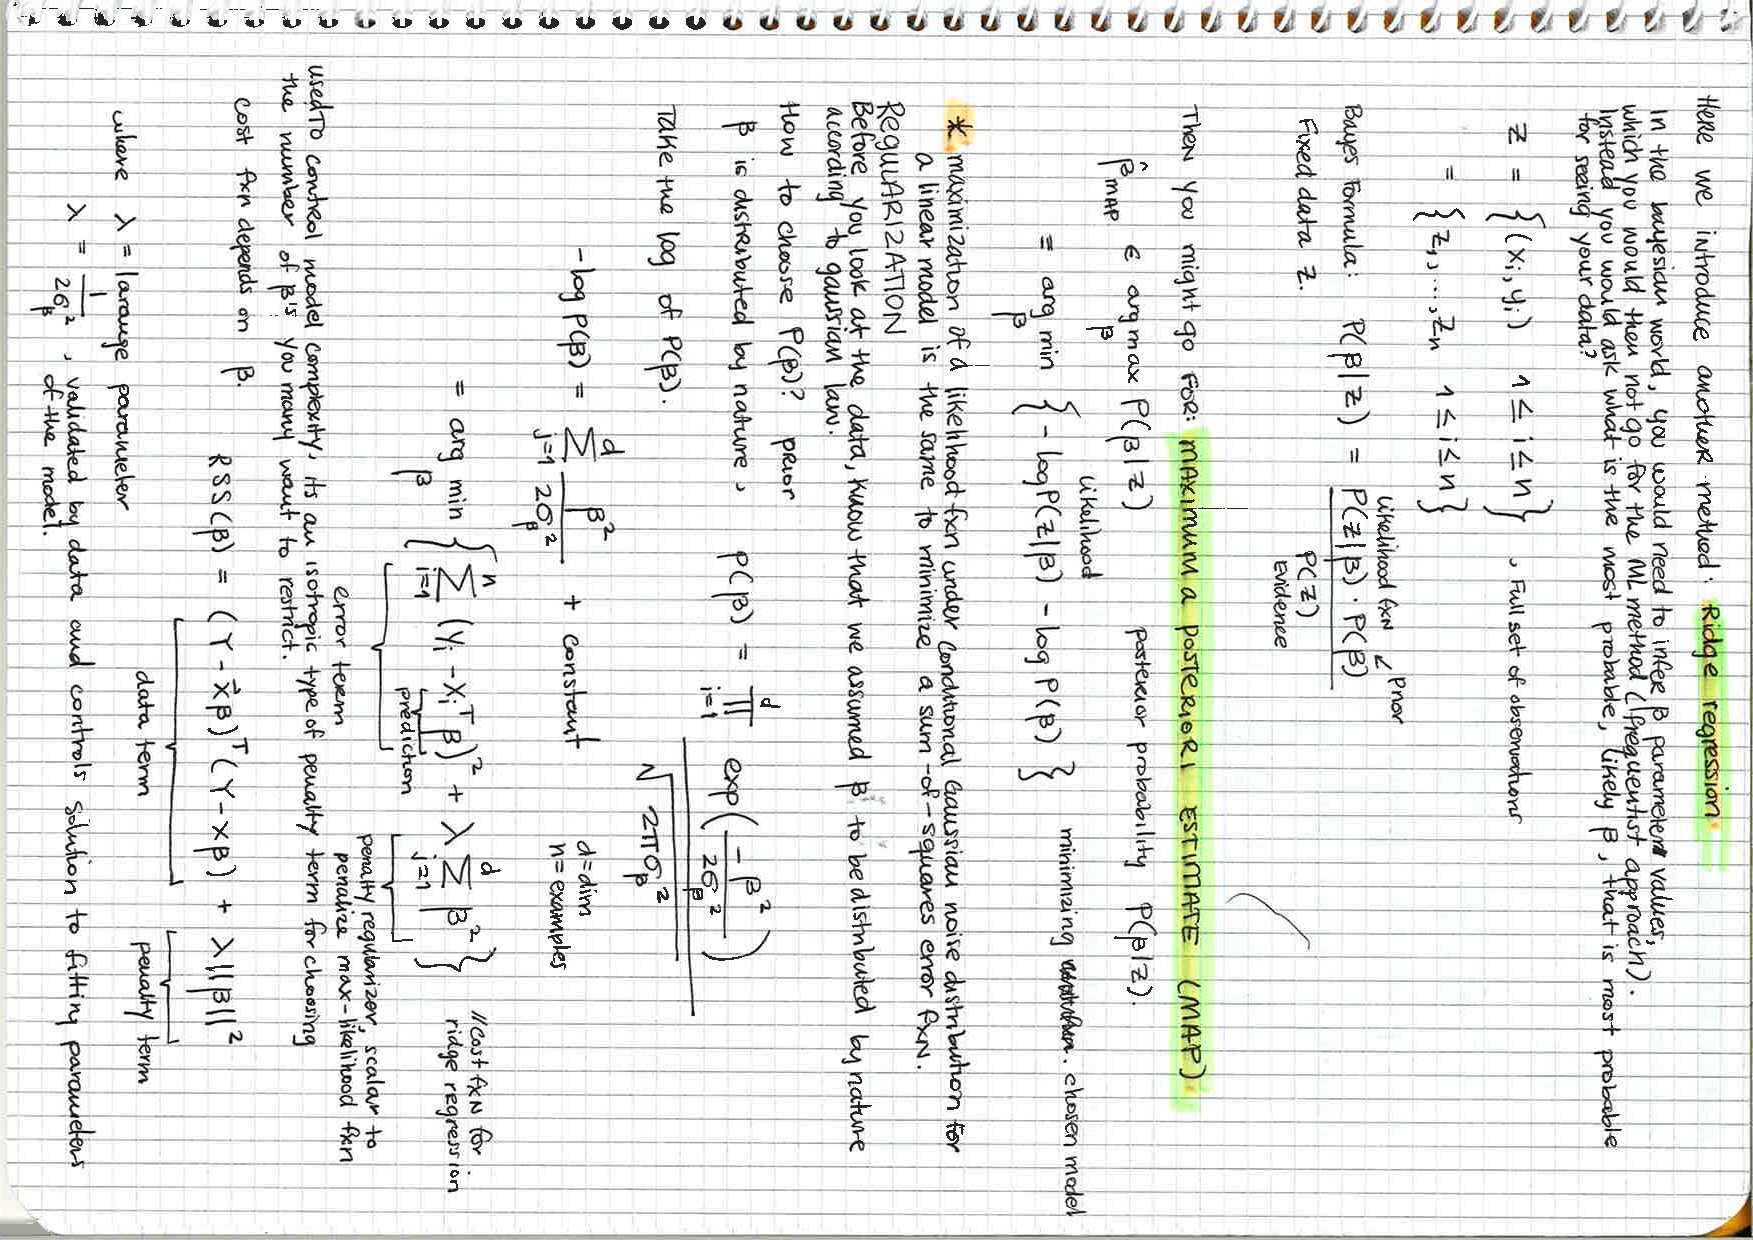
\includepdf[pages=1,angle=90]{figs/bayesian/1547_001.pdf}
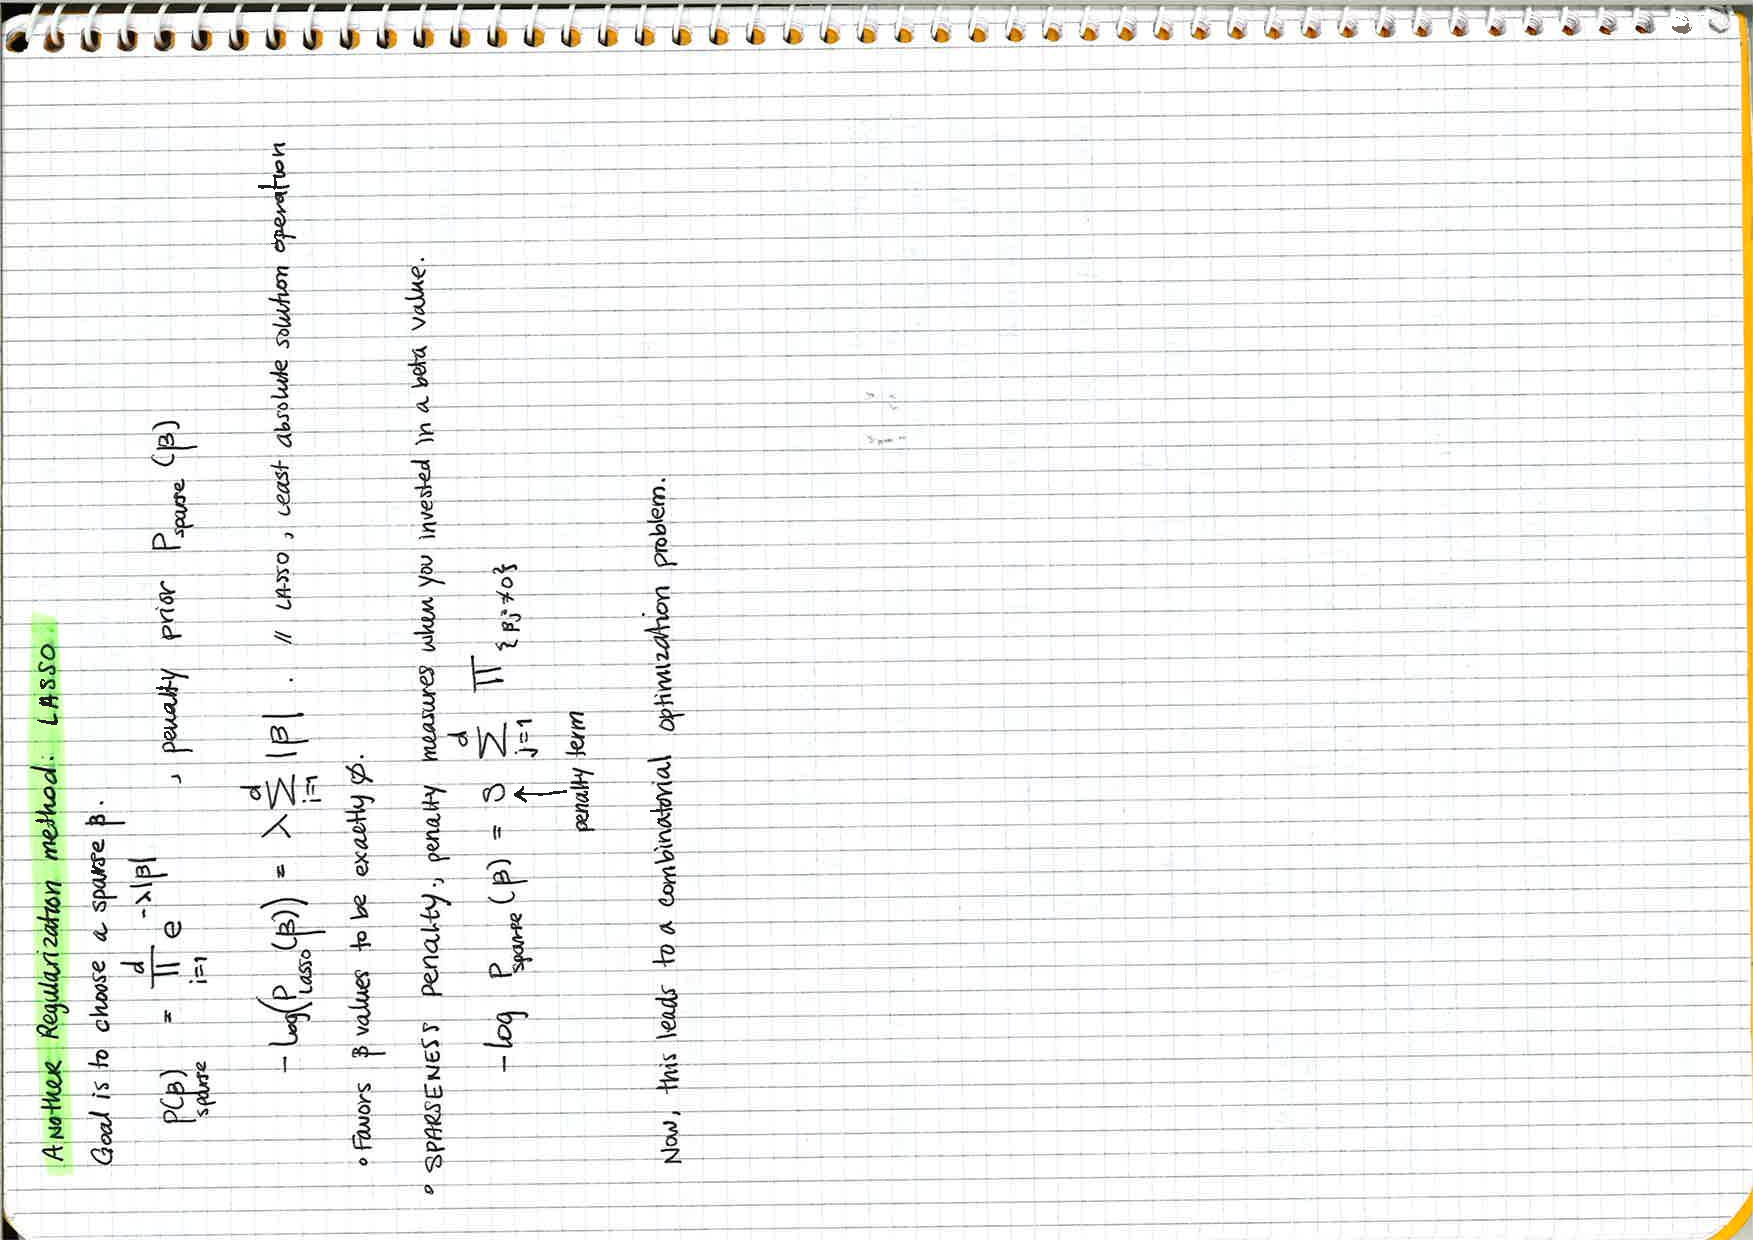
\includepdf[pages=1,angle=-90]{figs/bayesian/1548_001.pdf}
\todo[inline]{Probably somebody should tex the bayesian part of this at some point.}
\subsection{Readings}
\begin{enumerate}
\item Maximum Likelihood Estimators: Duda chp 3.1,3.2
\item Bayesian Estimator: Duda chp 3.3,3.4,3.5
\end{enumerate}
\end{document}